%%%%%%%%%%%%%%%%%%%%%%%%%%%%%%%%%%%%%%%%%%%%%%%%%%%%%%%%%%%%%%%%%%%%%%%%%%%
%% This file is part of the book
%%
%% Algorithmic Graph Theory
%% http://code.google.com/p/graph-theory-algorithms-book/
%%
%% Copyright (C) 2009--2011 Minh Van Nguyen <nguyenminh2@gmail.com>
%%
%% See the file COPYING for copying conditions.
%%%%%%%%%%%%%%%%%%%%%%%%%%%%%%%%%%%%%%%%%%%%%%%%%%%%%%%%%%%%%%%%%%%%%%%%%%%

\documentclass{article}

\usepackage{subfigure}
\usepackage{tikz}
\usetikzlibrary{external}
\tikzexternalize{isomorphic-graphs}

\begin{document}

\begin{figure}
%% cycle graph C_6
\subfigure[$C_6$]{
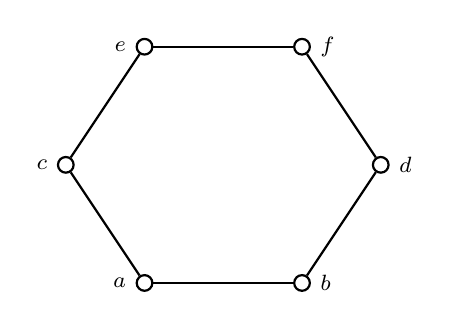
\begin{tikzpicture}
[lineDecorate/.style={-,thick},%
  nodeDecorate/.style={shape=circle,inner sep=2pt,draw,thick}]
%% nodes or vertices
\foreach \nodename/\x/\y/\direction/\navigate in {
  a/0/0/left/west, b/2/0/right/east, c/-1/1.5/left/west,
  d/3/1.5/right/east, e/0/3/left/west, f/2/3/right/east}
{
  \node (\nodename) at (\x,\y) [nodeDecorate] {};
  \node [\direction] at (\nodename.\navigate) {\footnotesize$\nodename$};
}
%% edges or lines
\path
\foreach \startnode/\endnode in {a/b, a/c, b/d, c/e, d/f, e/f}
{
  (\startnode) edge[lineDecorate] node {} (\endnode)
};
\end{tikzpicture}
}
%%
%%
\quad
%% graph G_1 that is isomorphic to C_6
\subfigure[$G_1$]{
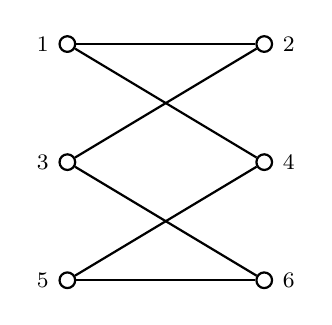
\begin{tikzpicture}
[lineDecorate/.style={-,thick},%
  nodeDecorate/.style={shape=circle,inner sep=2pt,draw,thick}]
%% nodes or vertices
\foreach \nodename/\x/\y/\direction/\navigate in {
  1/0/3/left/west, 2/2.5/3/right/east, 3/0/1.5/left/west,
  4/2.5/1.5/right/east, 5/0/0/left/west, 6/2.5/0/right/east}
{
  \node (\nodename) at (\x,\y) [nodeDecorate] {};
  \node [\direction] at (\nodename.\navigate) {\footnotesize$\nodename$};
}
%% edges or lines
\path
\foreach \startnode/\endnode in {1/2, 1/4, 3/2, 3/6, 5/4, 5/6}
{
  (\startnode) edge[lineDecorate] node {} (\endnode)
};
\end{tikzpicture}
}
%%
%%
\quad
%% graph G_2 that is non-isomorphic to C_6
\subfigure[$G_2$]{
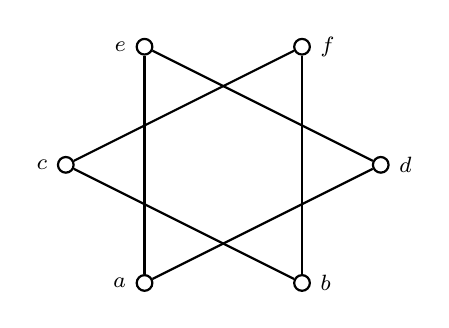
\begin{tikzpicture}
[lineDecorate/.style={-,thick},%
  nodeDecorate/.style={shape=circle,inner sep=2pt,draw,thick}]
%% nodes or vertices
\foreach \nodename/\x/\y/\direction/\navigate in {
  a/1/0/left/west, b/3/0/right/east, c/0/1.5/left/west,
  d/4/1.5/right/east, e/1/3/left/west, f/3/3/right/east}
{
  \node (\nodename) at (\x,\y) [nodeDecorate] {};
  \node [\direction] at (\nodename.\navigate) {\footnotesize$\nodename$};
}
%% edges or lines
\path
\foreach \startnode/\endnode in {a/d, a/e, b/c, b/f, c/f, d/e}
{
  (\startnode) edge[lineDecorate] node {} (\endnode)
};
\end{tikzpicture}
}
\end{figure}

\end{document}
